\documentclass[24pt, a0paper, portrait, margin=10mm, innermargin=5mm,
               blockverticalspace=0mm, blocktitlewidthratio=0.5, colspace=5mm, 
               subcolspace=5mm]{tikzposter} 

% Change font     
\renewcommand{\familydefault}{\sfdefault}

% LATEX PACKAGES
% --------------
  
\usepackage{graphicx}  % package for inserting images, including .pdf
\usepackage{adjustbox} % package for cropping images
\usepackage{url} % package for url 
\usepackage{wrapfig}
\usepackage{lmodern} %mix italic and bold
\usepackage{hyperref}% for url
\usepackage{authblk}
\usepackage{graphicx} 
\usepackage{caption}
\usepackage{mwe}
\usepackage[absolute]{textpos}
\usepackage{selinput}
\usepackage{multicol}
\usepackage{tikz}

% \usepackage{anyfontsize} %increase overall font size
\SelectInputMappings{%
  Lcaron={Ľ}
}

\definecolor{calpolypomonagreen}{rgb}{0.12, 0.3, 0.17}

% TITLE, AUTHORS, INSTITUTE
% -------------------------

\title{\textbf{\parbox{\linewidth}{\centering Reduced \textit{Eimeria} and pinworms loads in hybrid mice of the European house mouse hybrid zone}}}

\author[1,2,*]{\Large Alice~Balard}
\author[1,2]{Victor~Hugo~Jarqu\'{i}n-D\'{i}az}
\author[1]{Jenny~Jost}
\author[3]{Iva~Martincov\'{a}}
\author[3]{{Ľ}udov\'{i}t \v{D}ureje}
\author[3]{Jaroslav~Pi\`alek}
\author[4]{Milo\v{s}~Macholán}
\author[3]{Jo\"{e}lle~Go\"{u}y~de~Bellocq}
\author[3]{Stuart~J.E.~Baird}
\author[1,2]{Emanuel~Heitlinger}

\affil[1]{\large Institute for Biology. Department of Molecular Parasitology. Humboldt University Berlin, Germany}
\affil[2]{\large Leibniz Institute for Zoo and Wildlife Research, Berlin, Germany}
\affil[3]{\large Research Facility Studenec, Institute of Vertebrate Biology, Czech Academy of Sciences, Czech Republic}
\affil[4]{\large Laboratory of Mammalian Evolutionary Genetics, Institute of Animal Physiology and Genetics, Czech Academy of Sciences, Czech Republic}
\affil[*]{\textcolor{yellow}{contact: alice.cam.balard@gmail.com}\vspace{-2ex}% reduce space
}

\makeatletter
\def\maketitle{\AB@maketitle}
\makeatother

% THEME SETTING
% -------------
\usetheme{Simple}

\colorlet{titlebgcolor}{calpolypomonagreen}
\colorlet{blocktitlefgcolor}{calpolypomonagreen}


% HEAD
% ----

\begin{document}
\maketitle

% Context
% ----

\block{Testing parasite resistance in \textit{Mus musculus domesticus}, \textit{M. m. musculus} and their hybrids	
}
{\begin{itemize}
	   \item Parasite models: 
	    \begin{itemize}
	  		\item \textit{Eimeria} spp., obligate intracellular parasite (Apicomplexa: Coccidia). \textbf{High impact on host health expected}
	  		\item Pinworms (\textit{Aspiruluris tetraptera} and \textit{Syphacia obvelata}). \textbf{Low impact on host health expected}
	    \end{itemize}
	  \item Aim of the study: \textbf{Investigating hybrid susceptibility/resistance of house mice to parasites presenting different pathogenicity, using prevalence and intensity data in a new transect of the European house mouse hybrid zone}
  \end{itemize}
}	

% MATANDMET
% ----

\begin{columns} 
  \column{0.7} \block{Material \& Methods}{
    \begin{itemize}
     \item Sampling 660 mice over 4 years; Host genotyping (4-14 diagnostic markers) on a 0 to 1 scale (equal admixture hybrids = 0.5)
     \item \textit{Eimeria} load estimated by quantitative PCR
     \item Pinworm load estimated by count
     \item Modellisation of parasite load along hybridization index, test hybrid effect by maximum likelihood
     \item Logistic regression presence/absence of parasite in direction of the hybrid zone center
     \item Body condition = residuals body length/body weight. Modellisation of body condition along hybridization index, test hybrid effect by maximum likelihood, test difference between infected/non-infected
      \end{itemize}
  }
  \column{0.3} \block{}{
  
    \begin{tikzfigure}[]
               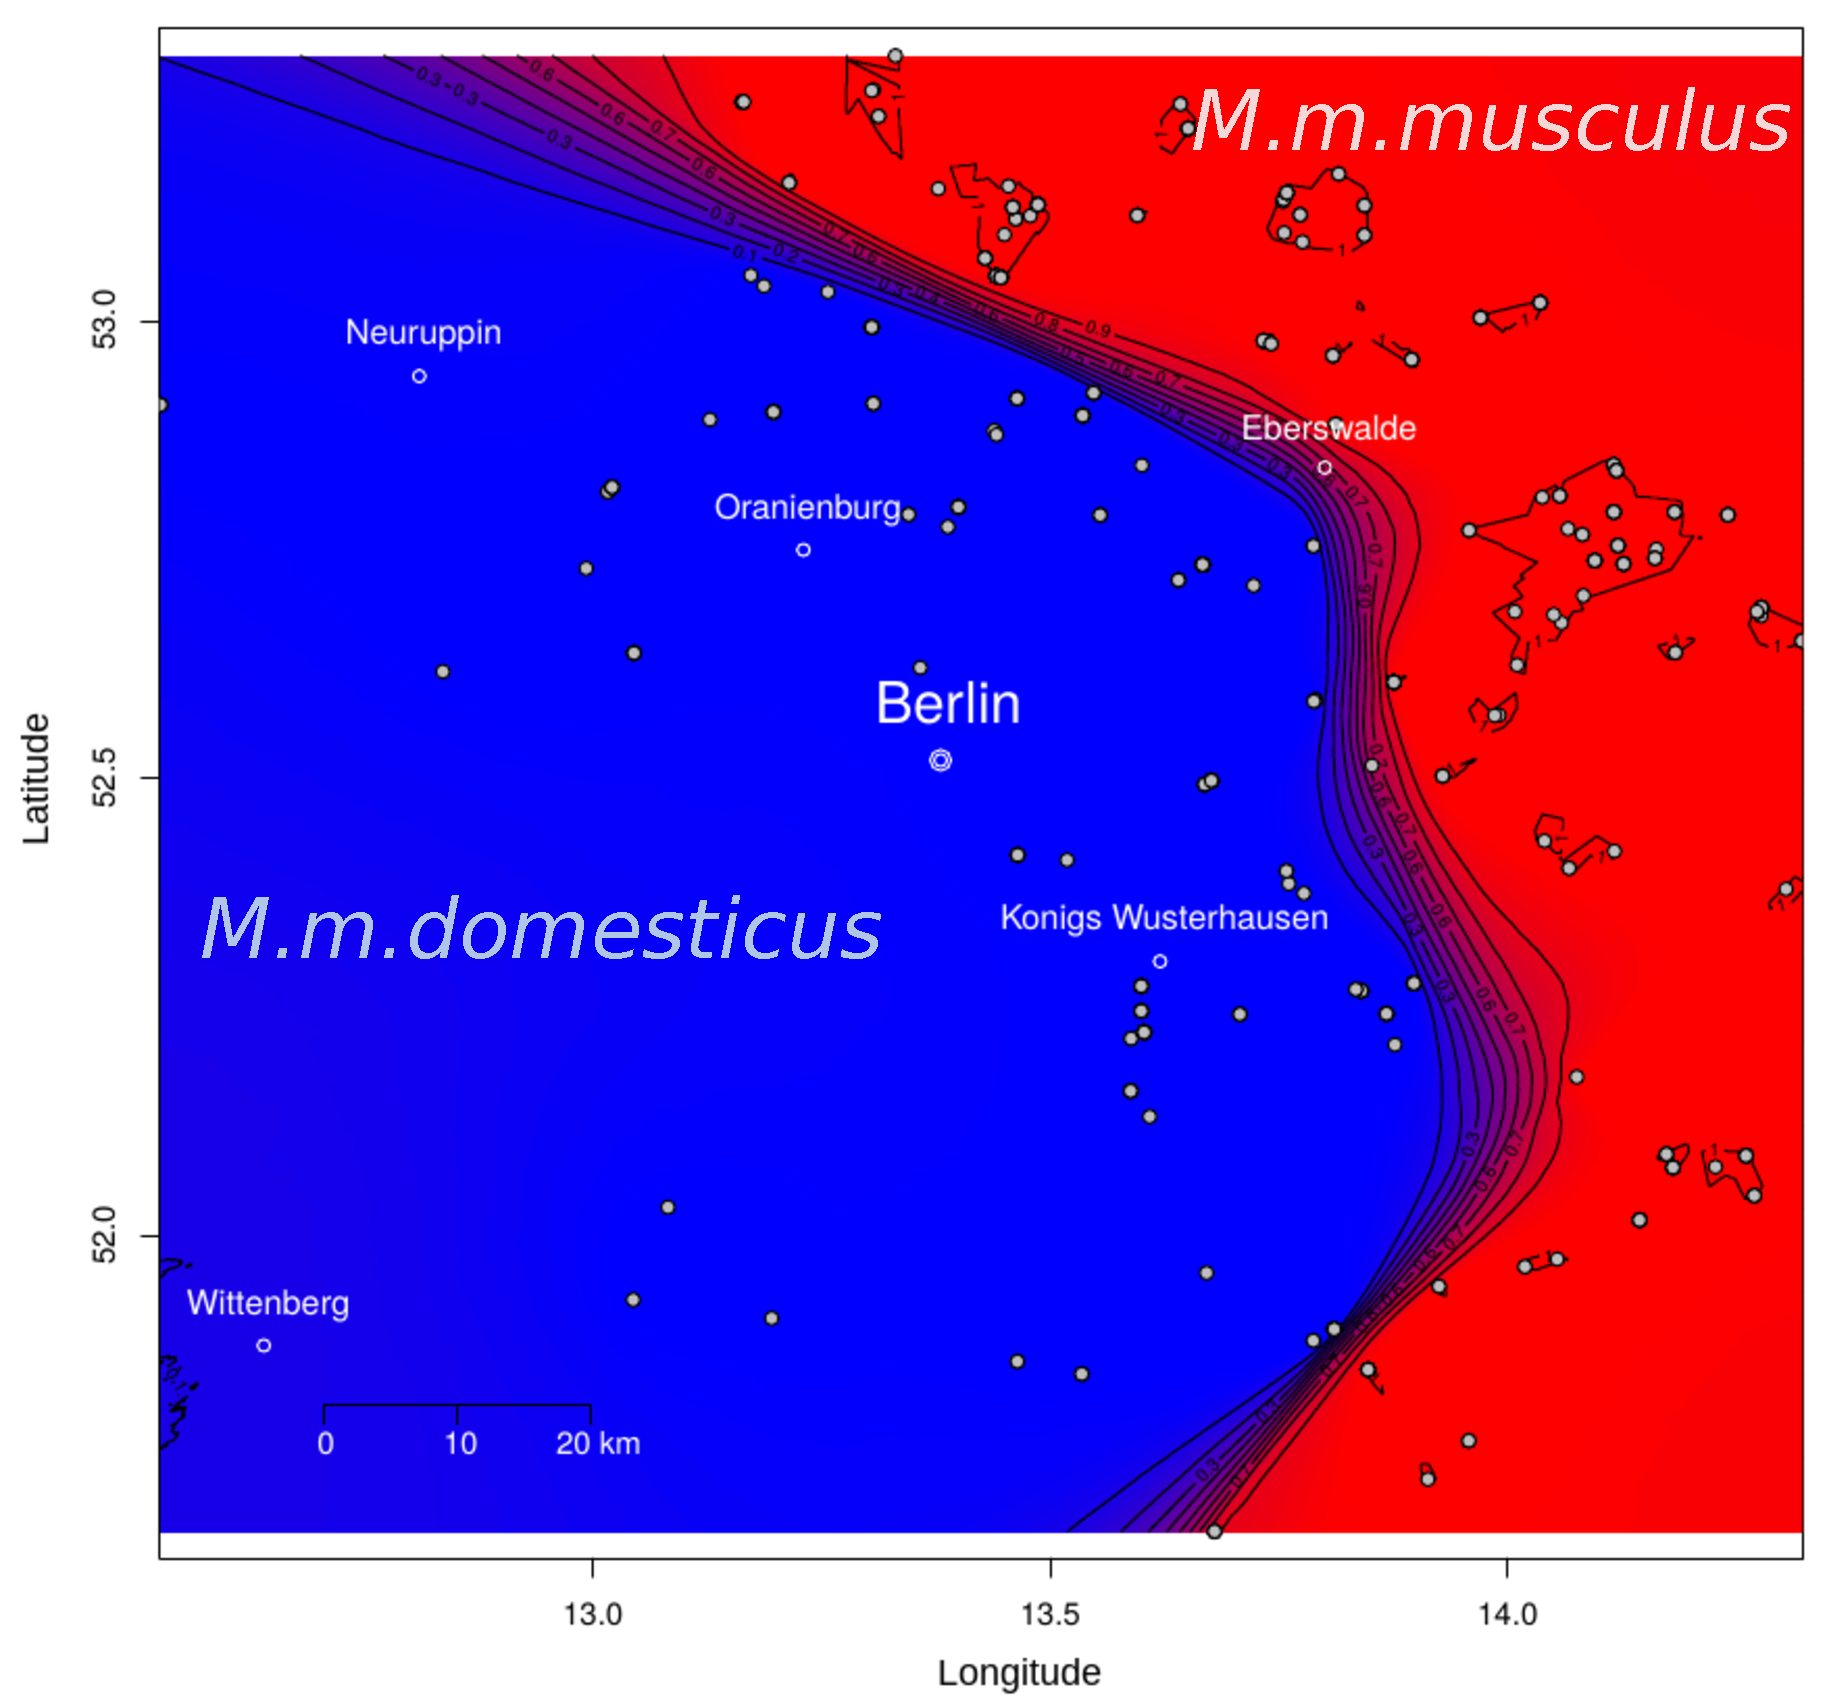
\includegraphics[scale=0.7]{Figure1.pdf}
    \end{tikzfigure}
    }
\end{columns}

% Results: parasite load
% -------

% Text and figure Inside the Block 
\block{\textit{Eimeria} spp. and pinworm loads are lower in hybrids than in parental mice}{
\begin{minipage}[t]{0.4\linewidth} 
\Large \centering \textit{Eimeria} \begin{tikzfigure}[] 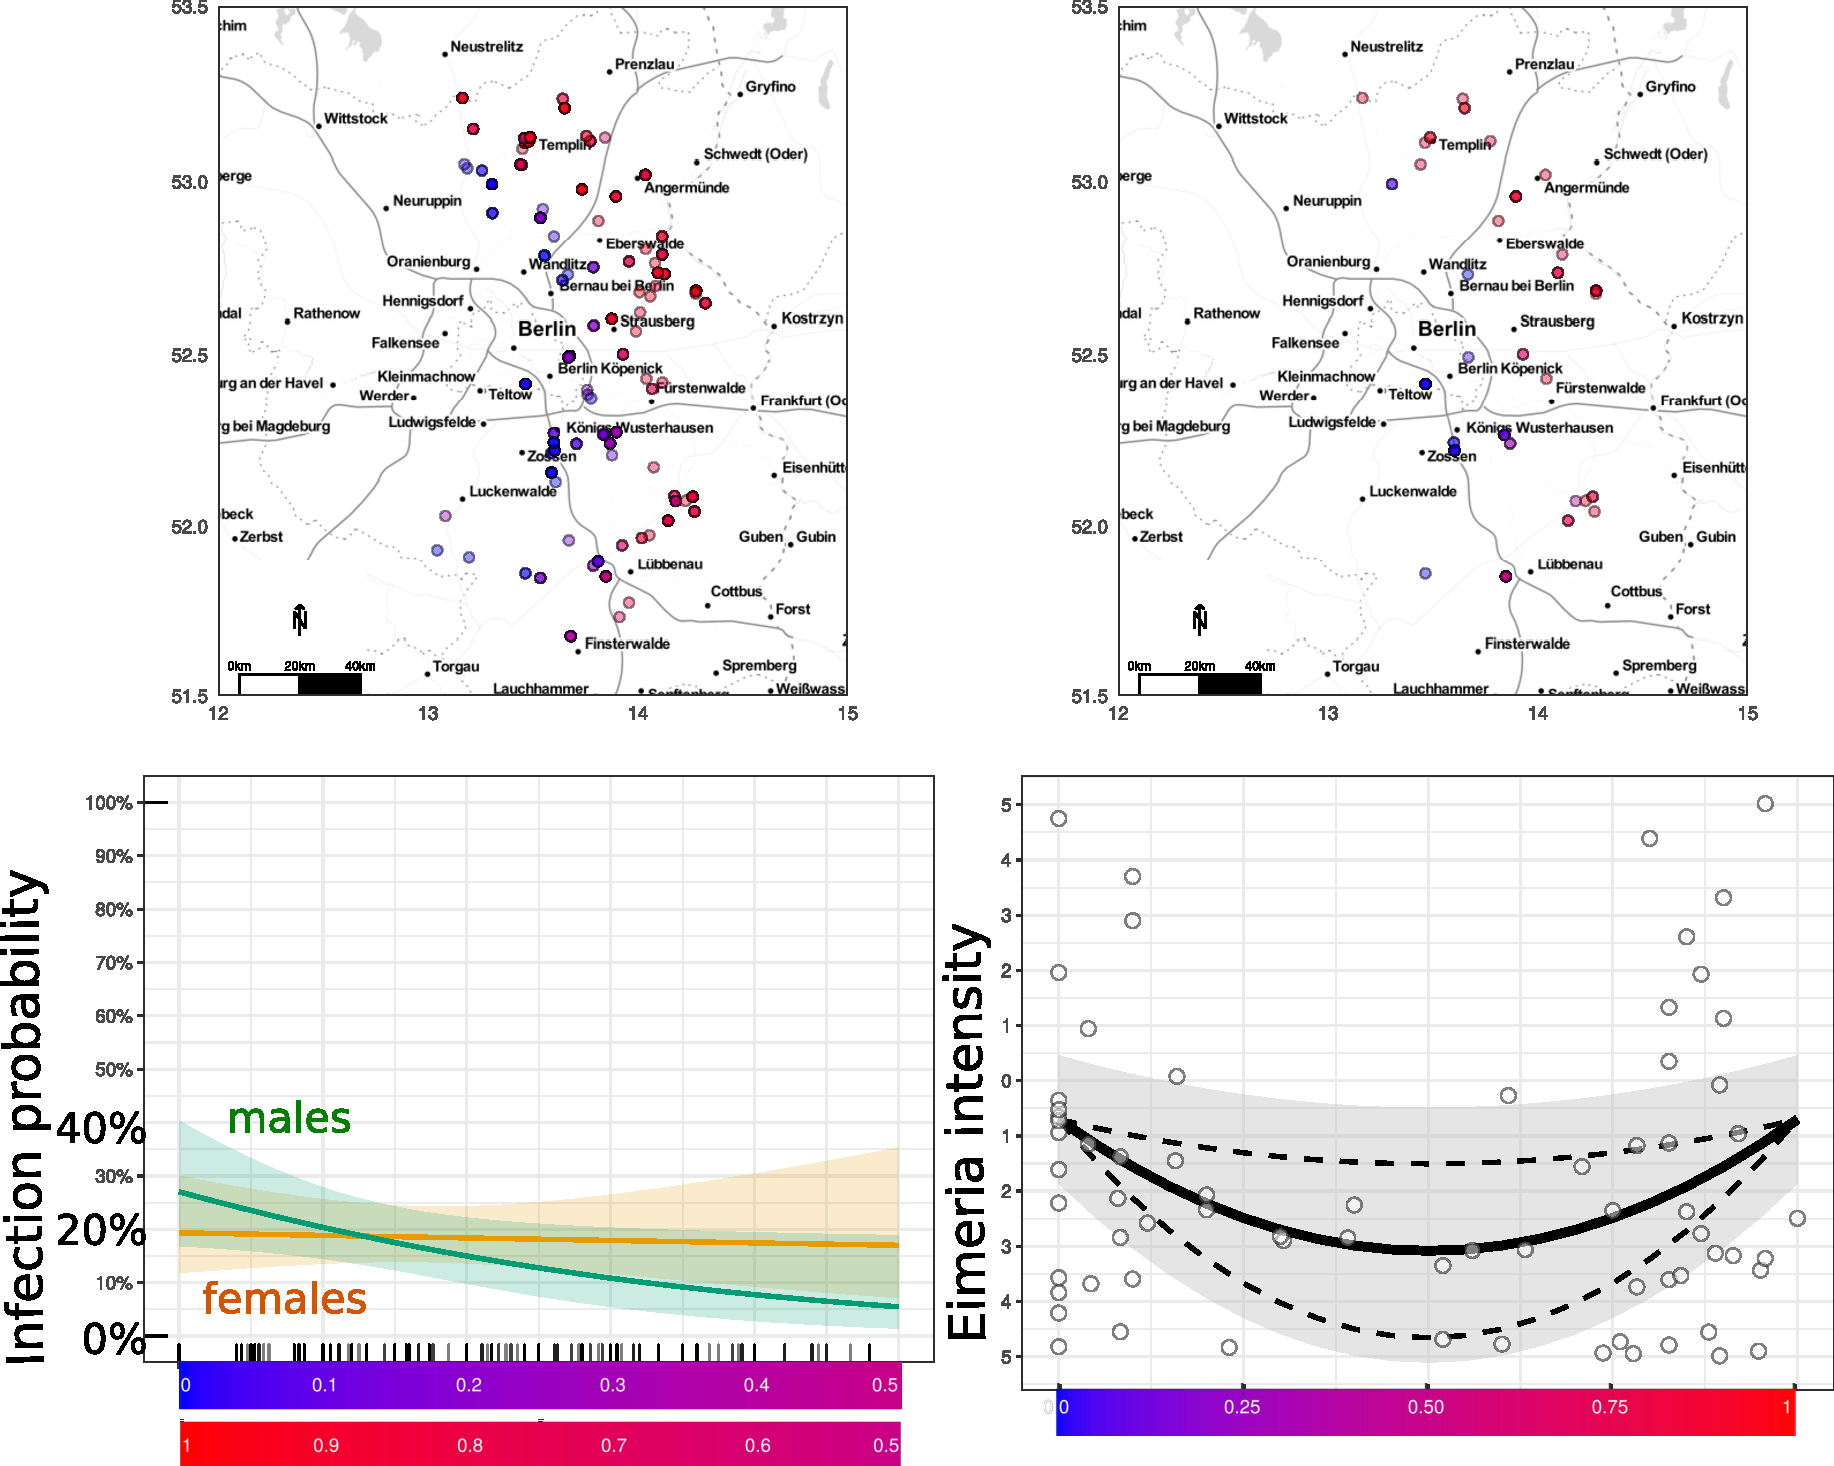
\includegraphics[scale = 1]{Figure2.pdf}
  \end{tikzfigure}
\end{minipage}% 
\begin{adjustbox}{valign=t} 
\begin{minipage}[t]{0.4\linewidth} 
\Large \centering Pinworms \begin{tikzfigure}[] 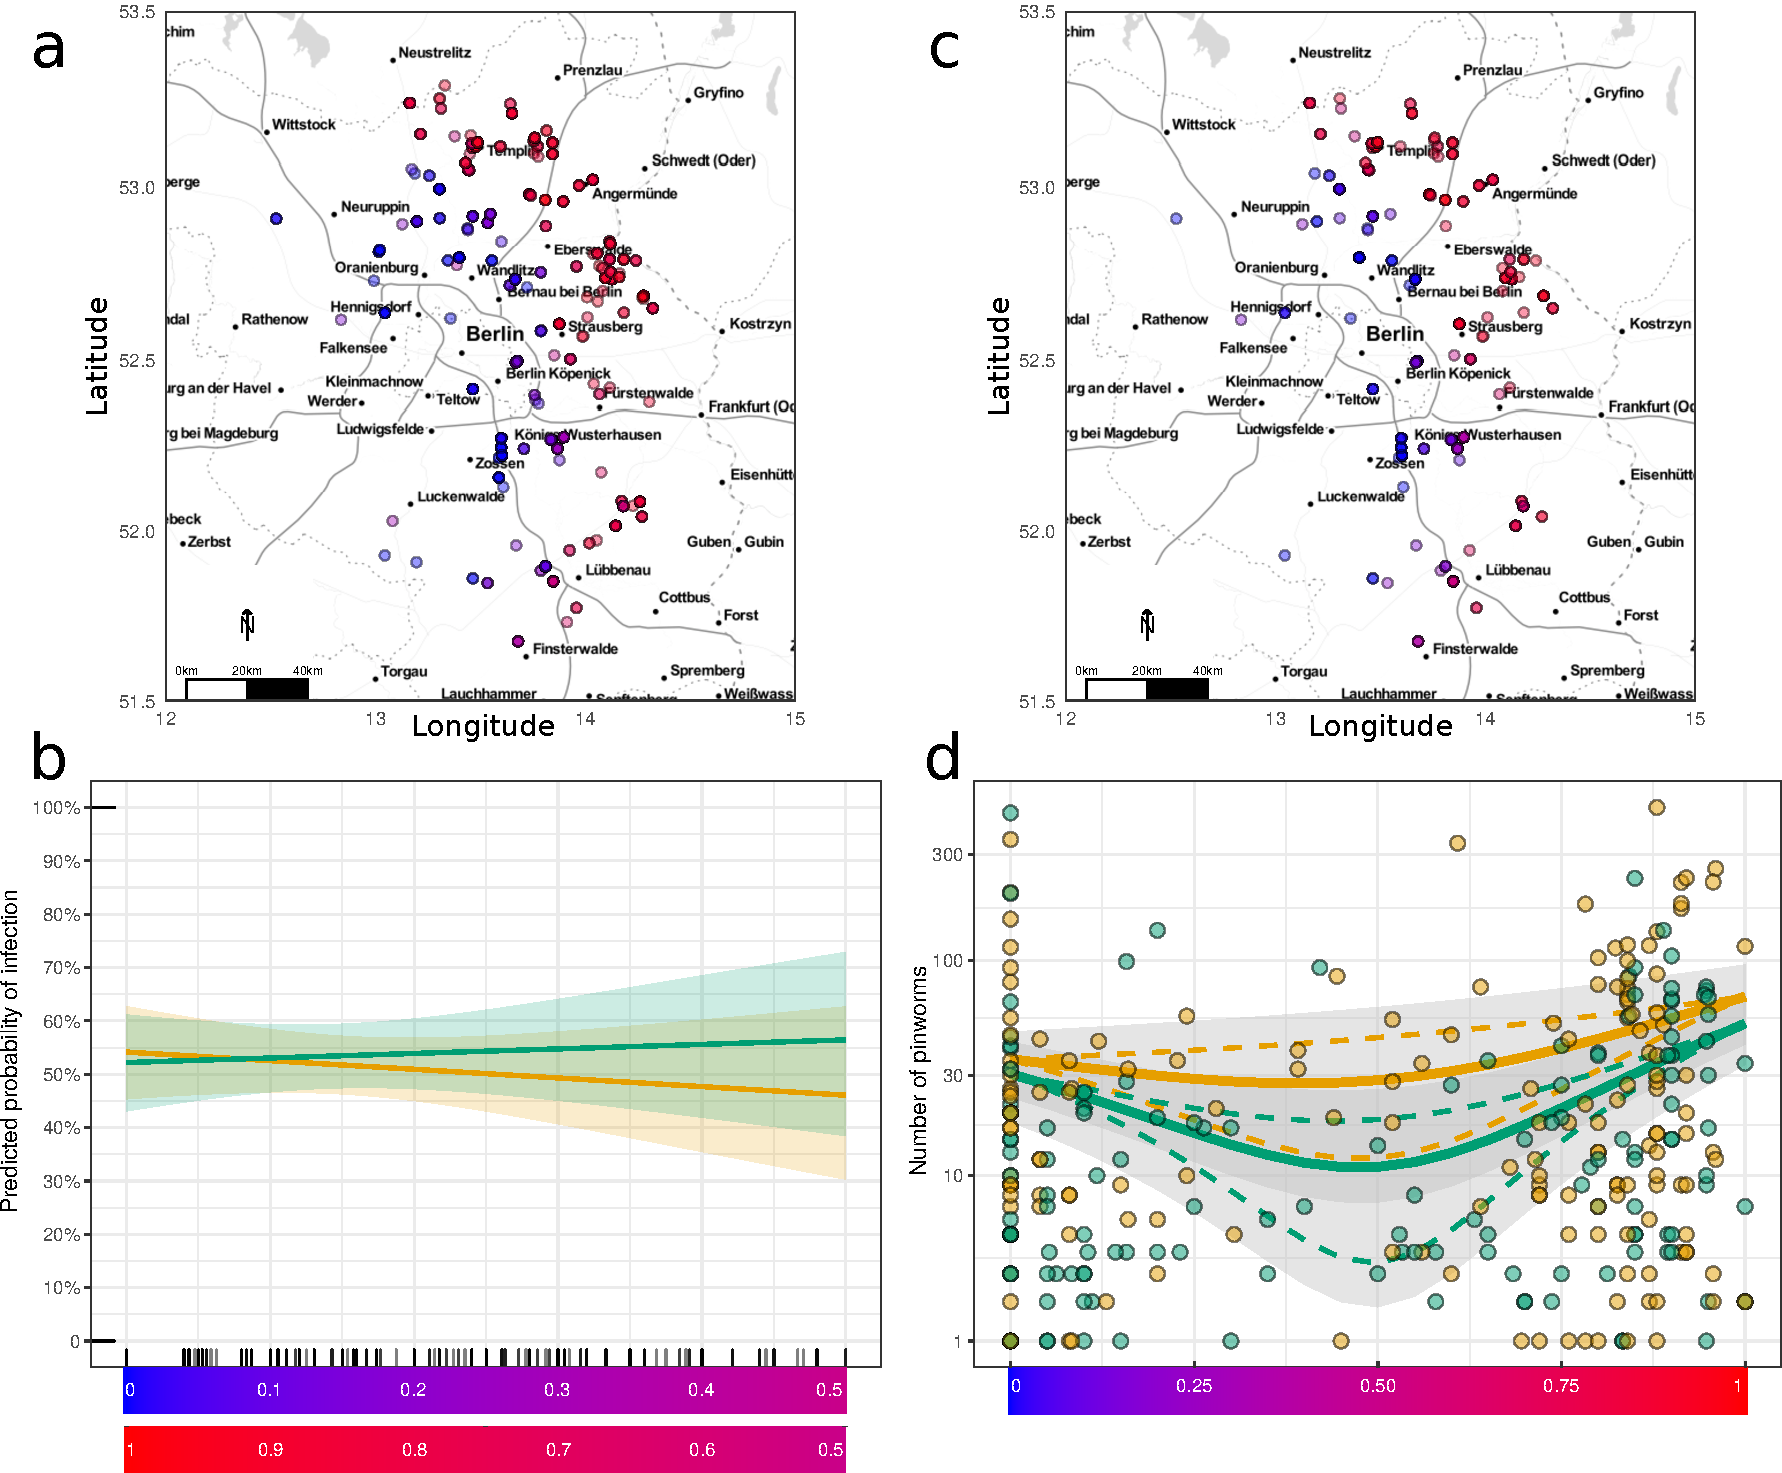
\includegraphics[scale = 1]{Figure3.pdf}
  \end{tikzfigure}
\end{minipage} 
\end{adjustbox}
\begin{adjustbox}{valign=t} 
\begin{minipage}[t]{0.2\linewidth} 
\Large \centering Mouse body condition \begin{tikzfigure}[] 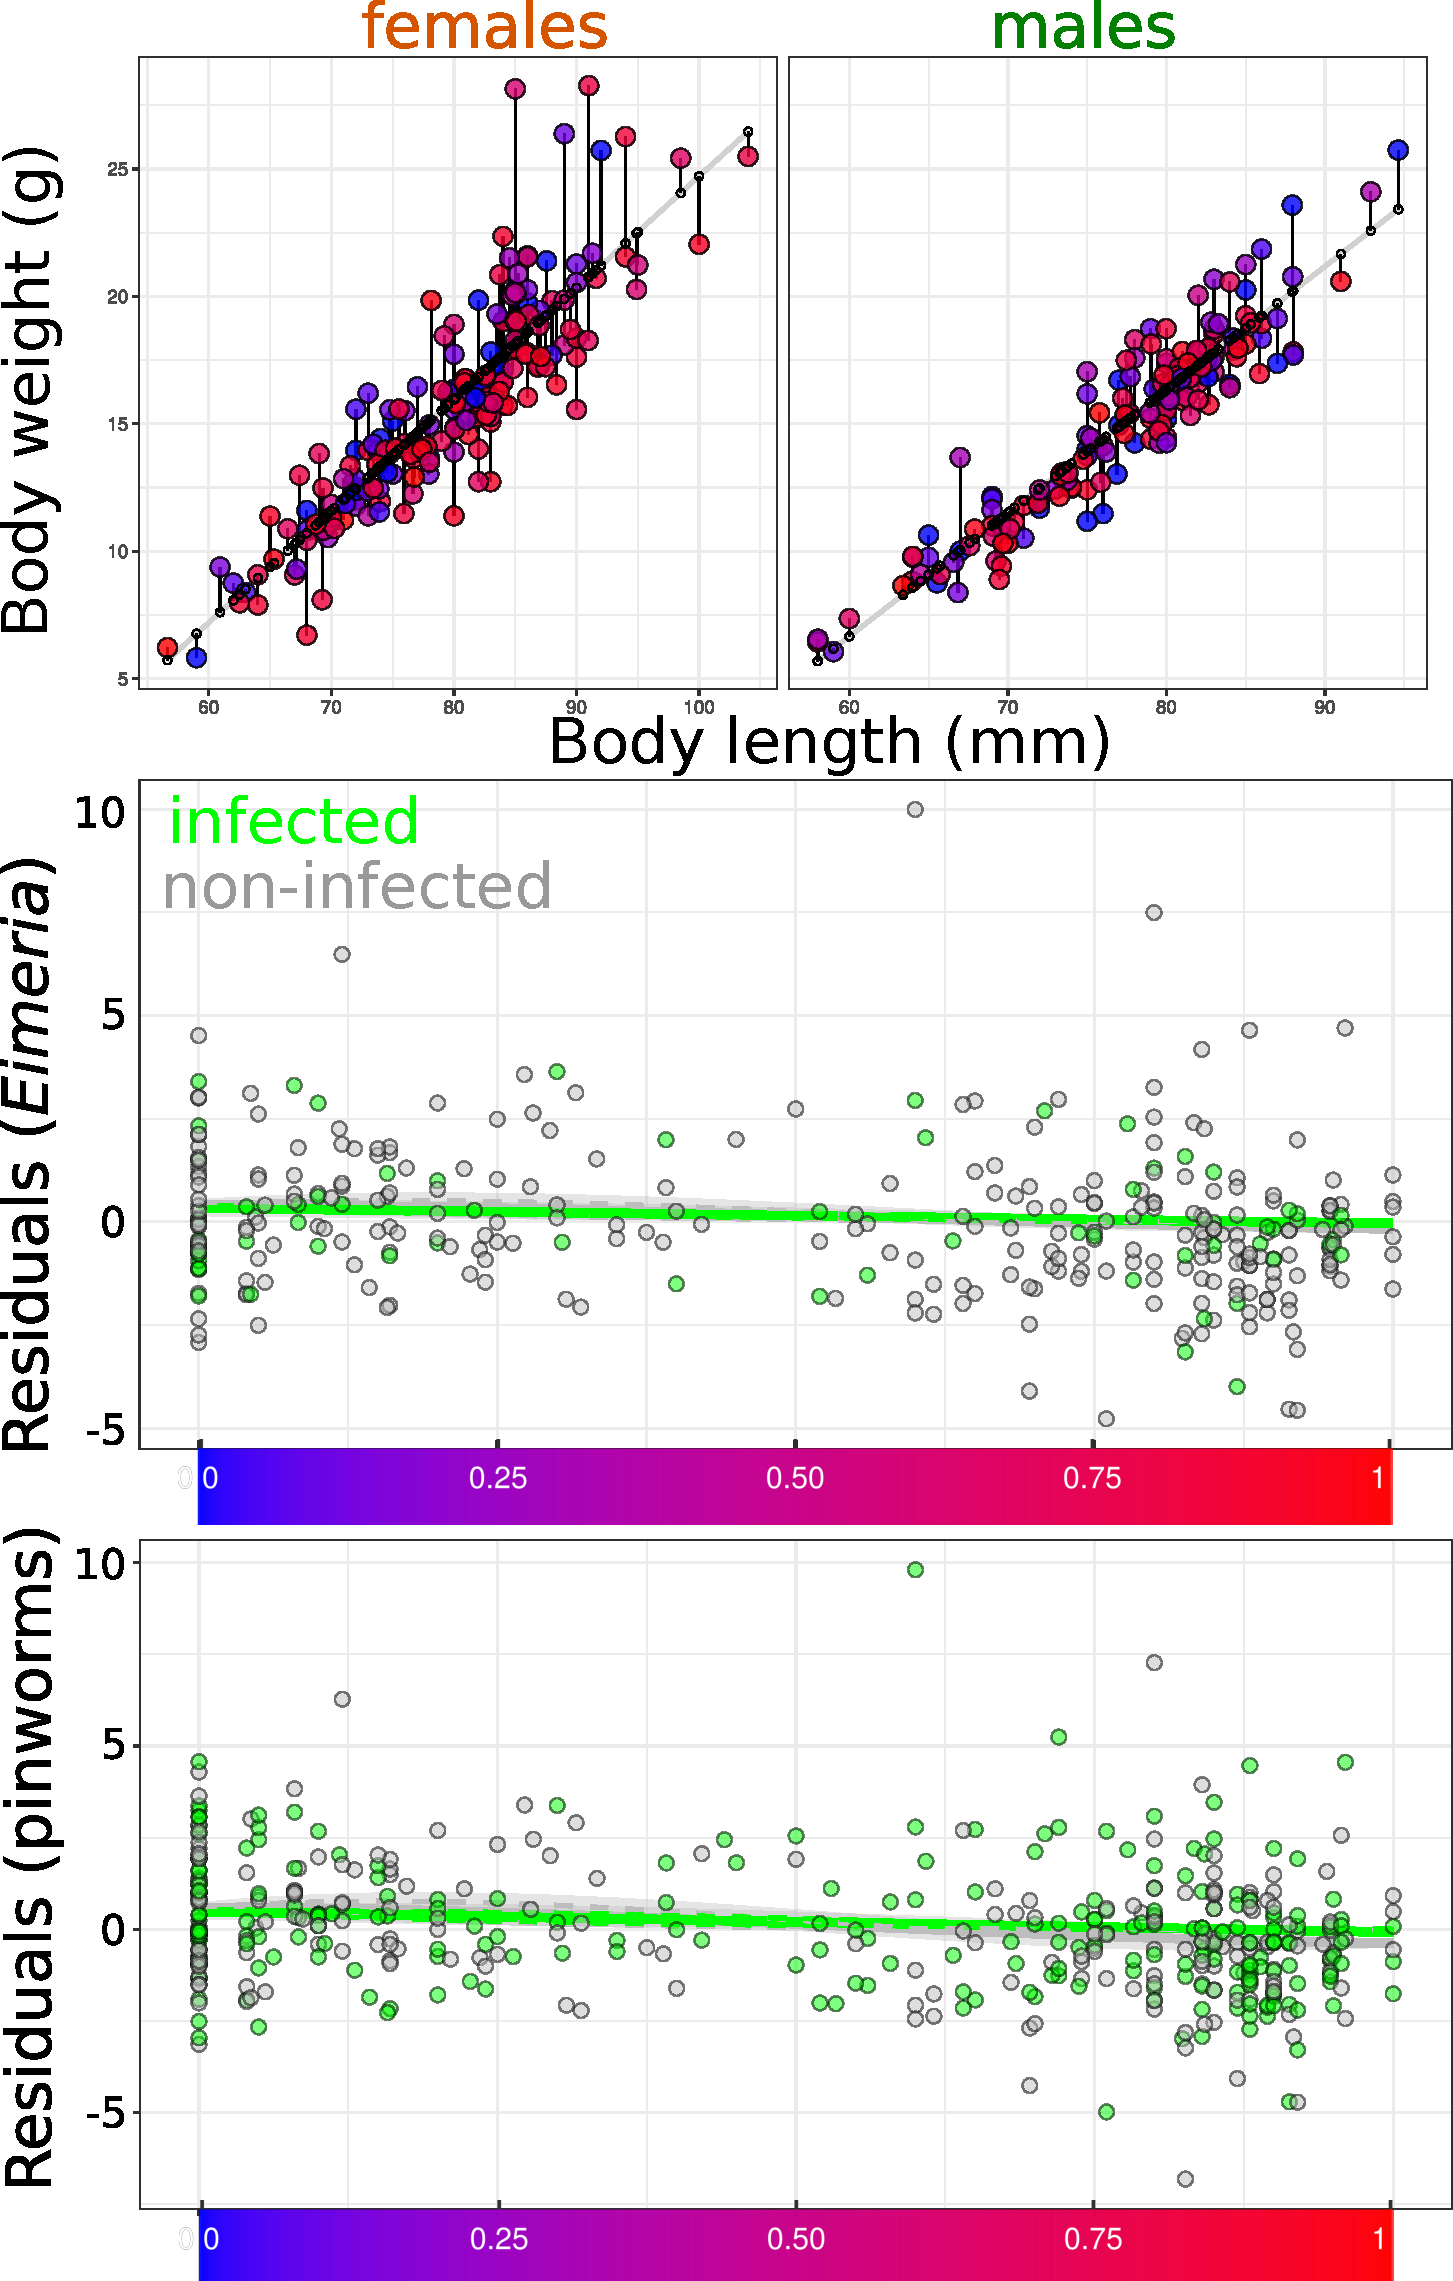
\includegraphics[scale = 0.65]{Figure4.pdf}
  \end{tikzfigure}
\end{minipage} 
\end{adjustbox} \\

\begin{itemize}
\item Similar parasite prevalence along the hybrid index
\item Statistically significant lower parasite load in the center of the hybrid zone
\item No indication of differential body condition between infected/non-infected / along hybrid gradient
\end{itemize}

} 

\block{Conclusion}
{
\begin{itemize}
  \item Increased resistance of hybrid mice compared to parental strains for both lower pathogenic parasite (pinworms) and high pathogenic one (\textit{Eimeria})
  \item Control for density troughs: no evidence of a lower parasite prevalence in the centre of the hybrid zone (exclude external ecological epidemiological factors)
  \item Independance of hybrid resistance from the parasite pathogenicity level
  
\end{itemize}
}

% REFERENCES
% ----------

\begin{columns} 
  \column{0.8} \block{References}{
Balard \textit{et al.} (unpublished) Reduced \textit{Eimeria} and pinworms loads in hybrid mice of the European house mouse hybrid zone \newline
R package used for modelling: Balard, A., and E. Heitlinger. 2019. Alicebalard/parasiteLoad DOI: 10.5281/zenodo.2535547
  }
  \column{0.2} \block{}{
    \begin{tikzfigure}[]
      
\includegraphics[scale=0.5]{AllLogos.png}
    \end{tikzfigure}}
\end{columns}

% ----------------
\end{document}
\endinput
%%
%% End of file 
